% Copyright (c) 2014,2016 Casper Ti. Vector
% Public domain.

\chapter{利用卷积神经网络分辨NLDBD事件和背景事件}
\label{chapter:cnn}

如上文所述,NLDBD 事件是一个极其稀有的事件,它的半衰期超过了 $1.07\times10^{26}$ 年,因而对于实验中的本底控制提出了很高要求。根据第\ref{chapter:background}章背景模拟得到的数据,PandaXIII 实验中 200kg 级探测器每年会有约 78 个本底 $\gamma$ 事件落在 ROI 能量区间中。这个背景事件率还是远远高于 NLDBD 实验的需求,因而需要一些其他的方式来压低本底信号,其中最自然的方法便是利用事件的径迹信息来区分背景事件和 NLDBD 事件。

NLDBD 事件会同时释放出两个高能电子,在其径迹的末端会有两个明显的布拉格峰,这便是 NLDBD 事件最为明显的径迹特征。传统的 $\gamma$ 本底事件一般通过一次或多次康普顿散射产生一个或多个次级电子,所以 $\gamma$ 射线会形成一个或多个单末端布拉格峰的径迹。如果我们能够重建得到事件的详细径迹信息,就可以由此高效的分辨出该事件是本底事件还是 NLDBD 事件,从而极大的压低本底。

然而因为 PandaXIII 读出系统的限制,使用传统的方法重建径迹会变得较为困难,因而我们探究了使用深度神经网络(DNN)中的卷积神经网络(CNN)来进行事件鉴别这一方法,得到了较为优秀的效果。本章节详细描述了利用 CNN 中进行事件鉴别的动机,CNN 模型的选择和搭建,数据处理和训练等细节,希望能够帮助读者建立起对于 DNN 以及 CNN 清晰简单的认识,为高能物理甚至是其他领域的研究提供相应的帮助。

\section{传统鉴别方法以及遇到的困难}

NLDBD 是一个径迹特征十分明显的事件,图\ref{fig:samples}给出了NLDBD 信号事件和 $\gamma$ 背景事件径迹的对比,可以很明显的看出NLDBD 事件径迹末端存在两个明显的布拉格峰,而背景 $\gamma$ 事件则只存在一个布拉格峰。如果 TPC 能够完美的重建出事件的径迹信息,那么鉴别该事件是否是 NLDBD 事件就会变得及其的简单:只要重建出事件沉积能量随径迹位置变化的关系,然后使用简单的 cut 就可以判断出该事件的类型。但是在 PandaXIII 中重建出完整的三维径迹十分困难,其原因如下。

\begin{figure}[hbt]
    \centering
    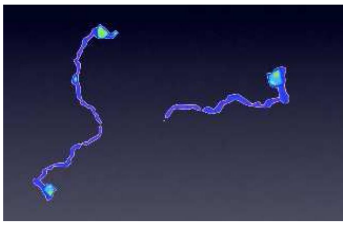
\includegraphics[width=0.5\columnwidth]{pic/fig10.png}
    \caption{一个 NLDBD 事件(左图)和一个 $\gamma$ 背景事件(右图)径迹投影示意图。可以很明显的分辨出左侧径迹末端有两个布拉格峰,而右侧只有一个末端有布拉格峰。}
    \label{fig:samples}
\end{figure}

PandaXIII 设计使用了 41 个 MM(Microbulk Micromegas)读出板来构建读出平面,每个 MM 板的尺寸为 20$\times$20 cm$^2$,按照图\ref{fig:mms}所示的结构排列组成,基本覆盖了整个读出平面,事件的读出效率相对较高。MM 板的结果如图\ref{fig:mm_detail}左所示,每个 MM 上都密布了许多增益孔(Amplification holes),用于采集漂移到附近的电子。多组增益孔按照合适的排布组成正方形的读出像素,每个像素的对角线尺寸约为 3 毫米。如果 MM 采取像素读出的话,每块 MM 需会形成 4000 个读出通道(channel),整个 TPC 所包含的通道数则会超过 32 万。后续电子学部分很难处理如此众多的通道,因而 PandaXIII 使用了条状读出来代替像素读出。如图\ref{fig:mm_detail}右图所示,每一组红色像素被连接在一起,在 Y 方向上形成 64 个通道,X 方向上同样由黄色像素组成 64 个通道。这样一块 MM 读出板只会形成 128 个通道,从而大大降低了后续电子学的复杂程度。

\begin{figure}[hbt]
    \centering
    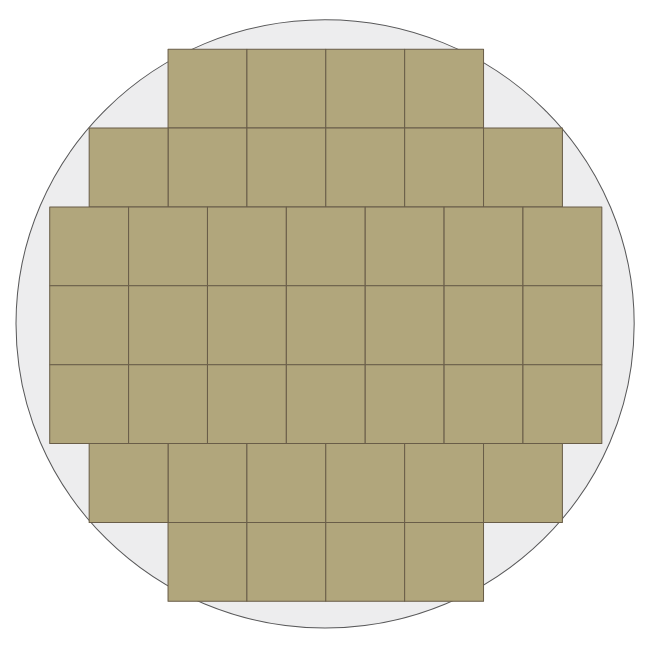
\includegraphics[width=0.4\columnwidth]{pic/fig8.png}
    \caption{41个 MM 板组合探测器读出平面排放示意图,按照 4,6,7,7,7,6,4层叠放置。}
    \label{fig:mms}
\end{figure}

\begin{figure}
    \centering
    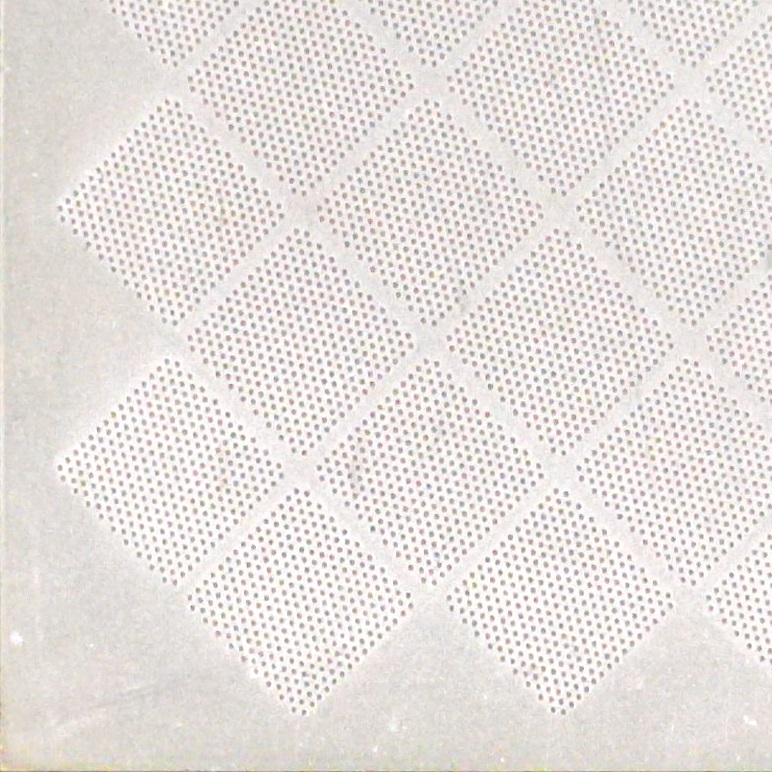
\includegraphics[width=0.4\columnwidth]{pic/MMStrips.jpg}
    \includegraphics[width=0.4\columnwidth]{pic/MMPattern.pdf}
    \caption{左图,MM 板局部读出区域的放大示意图,图中的小孔便是增益孔,若干孔组成一个菱形读出像素,每个像素的对角线长度约为 3 毫米。右图: MM 板局部读出通道连接示意图,红色或黄色正方形区域即为中图所示的读出像素,每一条红色虚线或者黄色虚线连接了一组读出像素,形成一个读出通道。\supercite{lin2018design}}
    \label{fig:mm_detail}
\end{figure}

但是采取条状读出也有一定的弊端,即我们无法同时获取到漂移到 MM 读出板上电子的 X 和 Y 的位置,只能得到它的 X \textbf{或} Y 的位置。加上通过漂移时间计算得到的 Z 方向上的相对位置关系后,一个事件的 X-Z-energy 和 Y-Z-energy 投影信息可以被快速的计算出,但因为有关 X-Y 的信息则因条状读出而被丢弃了。这就使得重建径迹的 3 维信息变得十分困难。

虽然一条比较直的径迹可以仅仅通过 X-Z 以及 Y-Z 来组合得到 X-Y-Z 的径迹,但是电子在 TPC 中的运动径迹往往不规则,同一时刻往往会有超过一组 X 和 Y 读出条被触发,这样同一 Z 值(同一时刻)的 X-Y 信息就无法确定。如图\ref{fig:difficulty_track_2}所示,如果两个真实的 hit 分别位于 ($x_1$,$y_1$) 和 ($x_2$,$y_2$),那么因为条状读出的原因,$x_1,x_2,y_1,y_2$ 所在的通道都会同时被触发,重建时就无法到底是哪两个点。图\ref{fig:difficulty_track}便给出一个难于重建的 NLDBD 事件投影图,该事件 Z 位于 80 到 110 毫米处的径迹纠缠在了一起,很难确定 X 和 Y 的对应关系。

\begin{figure}
    \centering
    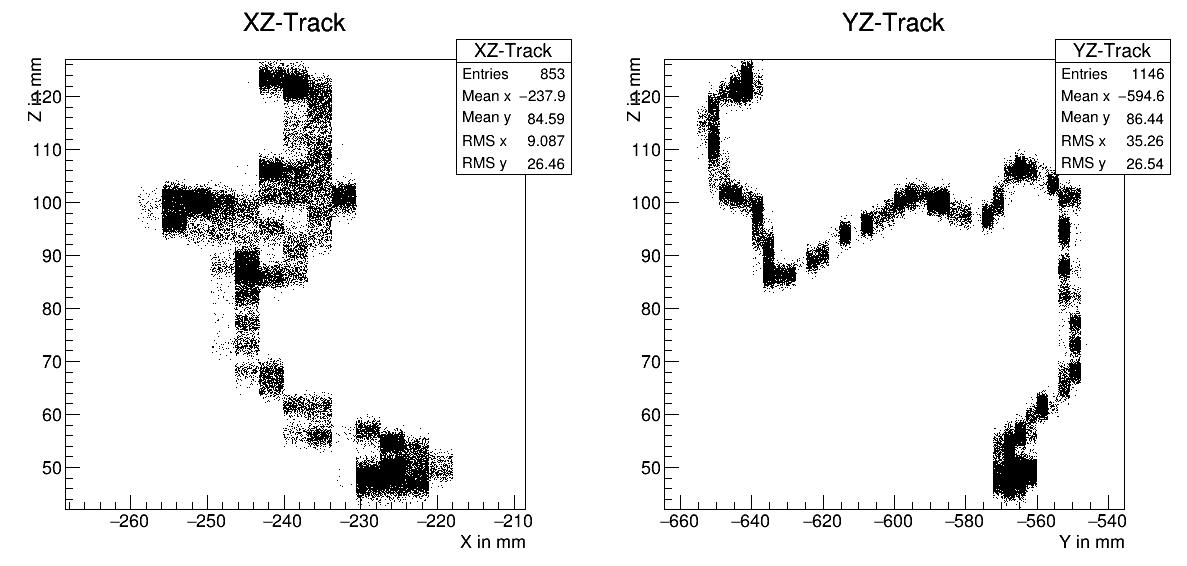
\includegraphics[width=0.7\columnwidth]{pic/difficulty_track.png}
    \caption{一个难于重建的事件的 X-Z-energy 投影和 Y-Z-energy 投影,区块深浅表示沉积能量的大小。Z 在 80 到 110 毫米内的径迹因为 X 方向上的多种可能而变得无法重建。}
    \label{fig:difficulty_track}
\end{figure}

\begin{figure}
    \centering
    \includegraphics[width=0.4\columnwidth]{pic/app01_strip_readout.pdf}
    \caption{条状读出易混淆原因的示意图。真实的能量沉积位置位于 ($x_1$,$y_1$) 和 ($x_2$,$y_2$),如图中绿色点所示。但是因为 $x_1,x_2,y_1,y_2$ 所在的通道同时被触发,所以也可能重建得到红色表示的错误位置。}
    \label{fig:difficulty_track_2}
\end{figure}

MM 的结构还带来了另外一个困难:因为一个电子只会落到 X 读出条或者Y 读出条所在的像素中的一个,所以同一个 hit 在两个投影上的能量并不相等,很难根据能量的大小关系来做 X-Y 之间匹配。作者个人认为在使用 MM 条状读出的前提下,基本不可能重建出完整的 3 维径迹,PandaXIII 实验需要寻找一种新颖的方法来进行事件鉴别。于是我们便试图将近年来在计算机领域大放异彩的深度神经网络引入事件鉴别中,以期望它能够解决这些问题。

\section{深度神经网络介绍以及使用动机}

\subsection{使用动机}

使用 MM 作为读出时很难通过重建出3维径迹后利用物理图像直接分类,但是如果将形如图\ref{fig:samples}的图片交于人眼来识别,那么可以相信通过简单训练我们可以轻而易举的分辨出 NLDBD 事件和背景 $\gamma$ 事件。在这个分辨过程中我们并没有试图将两个投影重建回 3 维的信息,而是直接通过分析比较它们的特征并直接找到径迹的末端。这种操作虽然可能通过精细的 cut 达成,但是在这些操作的过程中大量的信息会被丢弃以降低 cut 的复杂程度,从而可能影响鉴别的效果。

近年来随着机器学习技术的快速发展,一些深度神经网络(Deep Neural Network)似乎能够形成一些“智能”,例如 Google 公司所开发的围棋程序 AlphaGo\supercite{gibney2016google}就击败了诸多现役的围棋棋手,鉴于深度神经网络如此“智能“的表现,我们希望它能够完成类似与人所做到的事情,即通过观察径迹的两个方向上的投影而做出准确的判断。在各种深度神经网络中,有一类特别适应于图像分类处理的网络被称作卷积神经网络(Convolutional Neural Network)。CNN 能够直接将图片作为输入,所以如果使用它来进行事件鉴别的话便能够最大限度的利用重建得到的投影信息。同时我们可以通过蒙特卡洛模拟为 CNN 提供大量的信号样本和背景样本,在其他 CNN 应用场景中最为困难的样本采集和标定部分也就变得十分的简单。所以 CNN 非常适合 PandaXIII 实验粒子鉴别的需求,而事实上它也较为完美的达到了实验的目标,有关测试的结果见本章第\ref{section:cnn_result}节。

\subsection{神经网络介绍}

在神经网络的介绍之前需要先介绍一下机器学习。人们一直在探寻人类自身智慧的来源,从最开始哲学方面的探讨,再到近代从生物学医学的方向出发,智能一直是科学界中最令人着迷的一个方向。1949 年加拿大心理学家唐纳德·赫布提出了赫布理论\supercite{hebbian},为生物神经网络中的学习效应提出了理论上的解释。1952 年来自 IBM 公司的 Arthur Samuel 开发了一个国际跳棋程序,他发现他构造的这个程序能够随着局数的增多而下得越来越好,因此他给出了机器学习最初的定义,即”不需要显式编程就可以赋予机器某项能力的研究领域“。随后的几十年,机器学习领域一直在缓慢的发展,但也分化除了若干个方向,包括 1986 年由 J. R. Quinlan 提出的决策树,1995 年 Vapnik 和 Cortes 提出的支持向量机(Support Vector Machine,SVM)等\supercite{mlhistory}。直到 2008 年后,英伟达公司所提出的统一计算构架(Compute Unified Device Architecture,CUDA)\supercite{CUDA}的出现,使得人们利用计算机能够得到的计算能力极大地增强,机器学习中沉寂了多年的神经网络方向才得以快速的发展,重新回到了大众的视线。

神经网络(Neural Network)最基本的组织单元便被称为神经元(Neural)。每一个神经元都拥有着若干个输入,并通过一定的非线性算法将这些输入和自身存储的参数一起进行处理,给出一个或多个输出。简单而言,对于一组输入 $(x_1,x_2,...,x_n)$,神经元的第 $i$ 个输出的形式为:
$$ y_i= f(x_1,x_2,...x_n,a_{i1},a_{i2},...,a_{im})$$
其中 $(a_{i1},a_{i2},...,a_{im})$ 是神经元自身的参数,$f$ 为某一种非线性函数。实际上我们使用的神经元的结构相对简单,一个典型的全连接神经网络中的神经元如下所示:
\begin{equation}
     y=g(\omega_1 x_1+\omega_2 x_2 + ... + \omega_n x_n+ \omega_0))
     \label{eq:neural}
\end{equation}
式中 $(\omega_1,\omega_2,...,\omega_n)$ 被称作权重,$\omega_0$ 为偏置(Bias),$g(z)$ 被成为激活函数(Activation Function),激活函数的主要作用是为神经元提供非线性的成分。一个典型的sigmod 激活函数数学表达形式为:
$$g(z)=\frac{1}{1+e^{-z}}$$

一个神经元的输出可以当做另外一个神经元的输入,许多神经元共同组成一个网络,像生物的神经细胞一样相互影响,共同对输入量做出反应,这就是一个神经网络。然而为了简化模型通常会对网络进行分层研究。当若干个相似的神经元共同对一组输入做出反应时,我们可以将其称为一层网络,即 $\bar Y = F( \bar X, \omega_1,...,\omega_n)$ 其中输入便是一个张量(tensor) $\bar X$,输出则是另外一个张量 $\bar Y$。许多不同类型的层相互层叠,每一层的输出作为下一层的输入,最终形成一个形如:
\begin{equation}
    \bar Y_0 = \mathcal{F}(\bar X_0, \mathcal{W})
\end{equation}
的非线性系统。而神经网络的训练过程便是寻找最能够拟合已知输入输出的网络参数 $\mathcal{W}$。图\ref{fig:simple_nn}展示了一个简单的全连接神经网络示意图,该网络接受一个维度(shape)为3的张量作为输入,通过两层隐含层的处理后输出一个维度为1的张量(标量)。

\begin{figure}
    \centering
    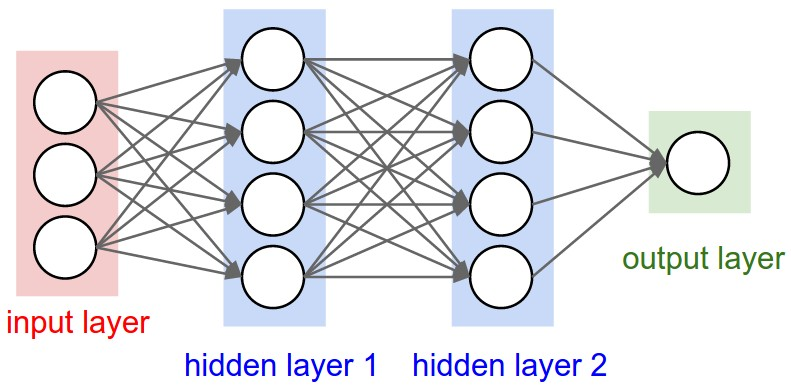
\includegraphics[width=0.7\columnwidth]{pic/simple_nn.jpeg}
    \caption{一个简易的全连接神经网络,包含一个输入层,两个隐含层以及一个输出层。}
    \label{fig:simple_nn}
\end{figure}

一个神经网络中所有神经元的参数便被称为该网络的权重(Weight),而神经网络中的层的类型和层的属性(神经元数目,组合方式)则被称作模型(Model)。如果我们要试图使用神经网络来解决问题,就需要按照下面的步骤进行:
\begin{enumerate}
    \item 确定网络的输入和输出,即明确问题的输入张量和输出张量分别是什么。
    \item 根据输入张量输出张量以及问题的特性构造合适的模型。
    \item 准备足够的输入输出样本数据。
    \item 使用合适的算法训练模型,得出最符合样本的权重数据。
    \item 使用该模型和训练得到的权重去预测未知的输入。
\end{enumerate}
在 PandaXIII 实验中,CNN 需要解决的问题是鉴别一个事件是 NLDBD 事件还是背景事件,这是一个非常明确的二分类问题,即输入是事件的信息,输出是事件的类型。然后我们可以按照上述的步骤,构建合适的模型,使用MC生成的数据对它们加以训练和测试,并将结果用于真实实验中。

\subsection{DNN,CNN以及其他类型神经网络介绍}

DNN 相对于传统神经网络最核心的区别便是网络层数多,结构复杂。虽然它的概念很早就被提出,但是直到2008年使用图形处理器加速通用计算的技术出现后,人们才有能力去训练使用深度神经网络。 一般来说拥有两个及以上隐藏层的网络便可以被称作深度神经网络,所以当今在图像处理人工智能等各个方向中所应用的神经网络基本上都可以称作 DNN 。但是在神经网络中,越是复杂的网络越需要细致的设计和优化调整来达到更为优异的效果,因此在处理具体问题中,相对从零开始构造一个 DNN 网络,尝试和修改现有的 DNN 网络更为可行。

CNN 是 DNN 极其重要的一部分,它广泛应用在图像识别的相关方向。相对于普通的全连接网络,CNN 的核心便是模型中拥有卷积层。一个简单的二维卷积操作如公式\ref{eq:con}所示。卷积神经网络处理的一般是图片,因而输入数据一般是一个二维的张量,它与一个被称作卷积核的参数矩阵做卷积操作,并将结果输出,这就形成了卷积层中的一个神经元。图\ref{fig:con}给出了另外一个卷积操作示意图。

\renewcommand\arraystretch{1.0}
\begin{equation}
    Input(\left[ \begin{array}{ccccc}
        1&1&1&0&0\\
        0&1&1&1&0\\
        0&0&1&1&1\\
        0&0&1&1&0\\
        0&1&1&0&0
    \end{array} \right])
    \otimes Convolutional Core(\left[ \begin{array}{ccc}
        1&0&1\\
        0&1&0\\
        1&0&1
    \end{array} \right]) = Output(\left[ \begin{array}{ccc}
        4 &3 &4\\
        2 &4&3\\
        2&3&4
    \end{array} \right])
    \label{eq:con}
\end{equation}

\begin{figure}
    \centering
    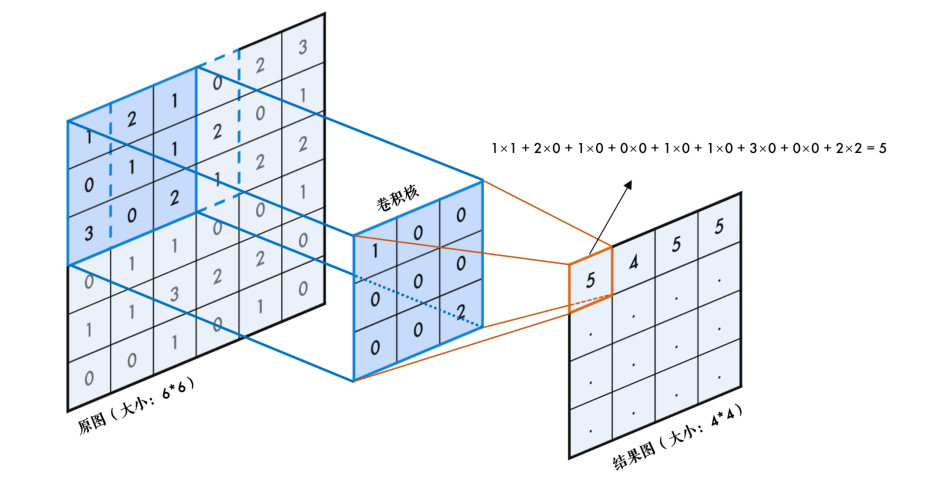
\includegraphics[width=0.7\columnwidth]{pic/con.jpg}
    \caption{一个卷积核部分卷积操作示意图\supercite{con}。}
    \label{fig:con}
\end{figure}

一层卷积层便是由$N$ 个卷积神经元所组成,每个卷积神经元都有一个 $M \times M$ 的卷积核。因而对于一个输入维度(X,X)的张量,卷积层使用了 $N\times M\times M$ 个参数对输入数据进行处理,输出张量的维度为 $(N,X-M+1,X-M+1)$。而如果试图使用全连接层网络寻找图片的 $N$ 个特征,那么全连接层的参数数目将会是 $N\times X\times X$ ,远远大于卷积层的参数数目。相对于全连接层,卷积层认为图片的局部特征是有一定的关联性和通用性的,所以可以以较小规模的卷积核来表示,并用卷积操作来提出该特征,从而在大大降低参数数目和计算复杂度的情况下依然拥有着良好的效果。

递归神经网络(Recurrent Neural Network, RNN)则更适用于自然语言处理等相关领域。相对于普通的全连接网络,递归神经网络考虑到了每一层内神经元之间的相互作用,即每次训练中递归层的结果会影响到下一次的训练过程中。因而递归神经网络可以提取数据序列中的相对关系,在自然语言处理,时间序列数据的处理更为合适。

对抗生成神经网络(Generative Adversarial Network,GAN)是一种特殊的训练网络方式,它同时训练两个网络模型,分别被称作生成模型和判别模型。生成模型用于从噪声中生成数据,判别模型则鉴别生成的数据和真实数据。通过对抗训练使得生成模型试图生成出判别模型无法区分的数据,而判别模型则努力鉴别出由生成模型生成的数据。因此 GAN 可以从既有的样本中提取特征,并依据这些特征创作新的数据。

\section{数据准备}
\label{section:data_prepare}

\subsection{输入数据和输出数据的格式}

使用 CNN 进行事件鉴别首先要明确问题的输入和输出。在 PandaXIII 实验中,我们希望它能够尽量多的利用既有数据,并由此给出事件的类型。根据探测器的读出结构以及先前进行的模拟工作,我们可以快速的重建出一个事件在 X-Z-energy 以及 Y-Z-energy 这两个方面上的投影信息,所以可以将这两个投影合并成一张图片作为网络的输入。网络的输出则是一个在(0,1)范围内的小数,代表着网络认为该事件更类似于一个背景事件(0)或者是一个信号事件(1)。

PandaXIII 实验中读出电子学部分将会以 5MHz 的频率采样 512 个时间点,即采样 $102\mu s$ 的数据,而电子在气体中的漂移速度为 1.87 mm/$\mu$s,那么一次触发探测器在Z方向上最长可以获取约 190 毫米的数据。MM 读出在 X 及 Y 方向上的像素尺度为 3 毫米,考虑到无论是NLDBD事件还是背景事件,它们在探测器中的径迹应该是各项同性的,即数据中 X,Y,Z 的地位也是一致的。因此我们认为转换完成的图片尺寸最大不超过63个像素,每个像素都代表着 $3\times 3$mm$^3$ 的区域。最终为了方便本文决定使用 $60\times60$ 像素的图片作为 CNN 网络样本图片。

每个事件重建后都会得到两个投影,而 CNN 一般只接受一张图片作为输入,因此我们需要将两个投影所转换出的两张图片合并成一张。每个投影都可以转换出一张灰度图片,而 CNN 神经网络可以接收彩色图片作为输入,所以可以将 X-Z-energy 投影转换出的灰度图片数据放置在红色通道中,Y-Z-energy 投影放置在绿色通道,如此操作就可以将两张灰度图片转换为一张彩色图片,从而用于 CNN 的训练和识别。同样的方法也被 NEXT-100 实验所采用\supercite{renner2017background}。

\subsection{NLDBD事件及背景事件的模拟数据生成}
\label{chapter:generate_nldbd}

在明确 CNN 网络的输入和输出之后便需要去准备样本以供 CNN 训练和测试。虽然 NLDBD 事件至今没有被探测到,但是依然可以根据相关的理论来推算出它的具体信息。在 PandaXIII 实验中我们使用了 DECAY0 软件包\supercite{ponkratenko2000event}来生成 NLDBD 事件发生后释放出的两个电子的动量信息,并将其作为 BambooMC 模拟框架的输入随机放置于灵敏气体中。通过和章节\ref{chapter:background}中的模拟工作相类似操作,可以得到 NLDBD 事件在探测器中 hit 的相关信息,其沉积能量能谱如图\ref{fig:nldbd_energy}左所示。

\begin{figure}
    \centering
    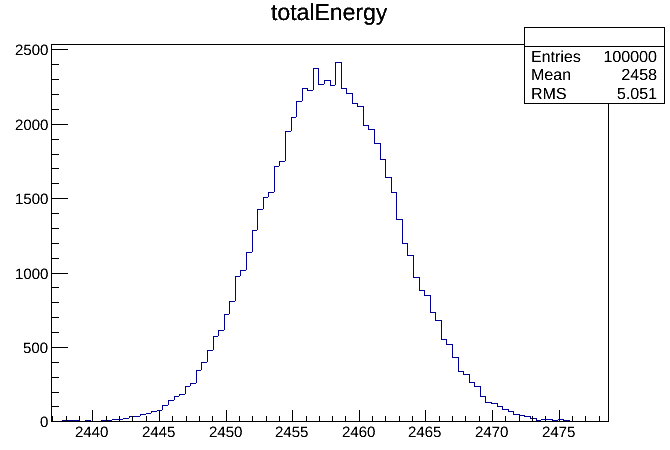
\includegraphics[width=0.3\columnwidth]{pic/nldbd_raw_spectrum.png}
    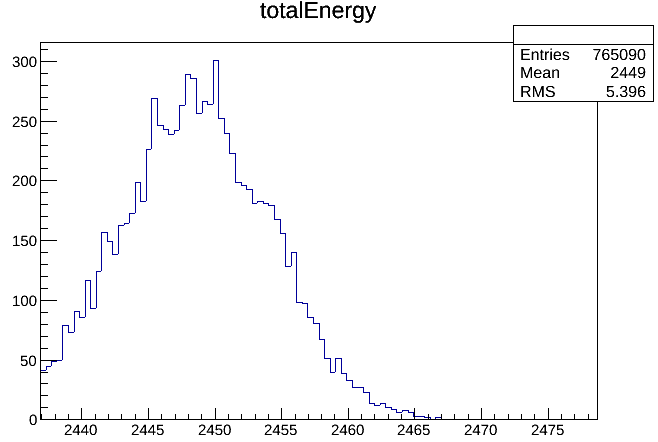
\includegraphics[width=0.3\columnwidth]{pic/2447_raw_spectrum.png}
    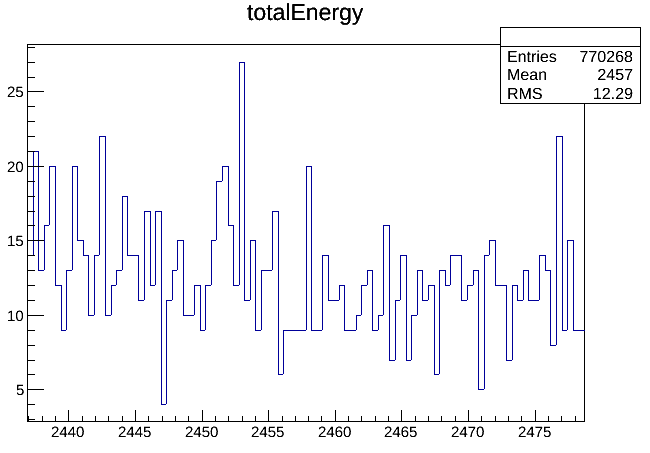
\includegraphics[width=0.3\columnwidth]{pic/2614_raw_spectrum.png}
    \caption{为 CNN 准备样本时使用 BambooMC 模拟出的事件能谱图。左: NLDBD 事件,中: 2447keV $\gamma$ 本底事件,右: 2614keV $\gamma$ 本底事件}
    \label{fig:nldbd_energy}
\end{figure}

对于背景事件而言,因为在 CNN 训练中需要准备大量的背景数据,像背景模拟一样进行 \utte 和 \thttt 全链模拟的时间代价过于高昂。同时因为探测器背景事件主要是来自于 $^{214}$Bi 的 2447.8keV 以及 $^{208}$Tl 的 2615.keV $\gamma$ 射线,所以可以直接将这两个能量的 $\gamma$ 粒子放置在探测器的铜罐中作为起始事件进行模拟,其能谱如图\ref{fig:nldbd_energy}中图和右图所示。在这里我们做了两个近似,即使用两个 $\gamma$ 事件代替真实的 \utte,\thttt 本底事件,以及使用铜罐作为事件的起始位置。第一个近似的原因有两点:我们猜测 CNN 神经网络是通过识别图片特征而不是通过事件的总能量来判断类型;在将事件投影转换为图片的过程中进行了归一化操作,丢弃了事件总能量的信息。第二个近似的原因也有两点: $\gamma$ 射线穿透能力相当强,其被探测器探测到的位置于它的起始位置关系不大;在将事件投影转换为图片时 hit 的绝对位置信息被丢弃了。这两点近似在后续测试结果的过程中都进行了相关的验证,可以参见章节\ref{section:cnn_result}。

\subsection{模拟数据转换为图片}

后续的处理过程如图\ref{fig:process}所示,在 BambooMC 模拟得到背景和信号的 hit 信息后,我们依然需要像探测器背景模拟中一样考虑探测器响应,MM 的结构以及电子学读出设计对于事件的影响,依次将蒙特卡洛得到的原始 hit 信息转换为电子学读出得到的每个通道波形信息。随后再通过读出系统道数和位置的关系重建出事件的 X-Z-energy 以及 Y-Z-energy 投影,并最终将其合并转换为图片供CNN神经网络所使用。各个转换步骤的细节如下:

\begin{figure}
    \centering
    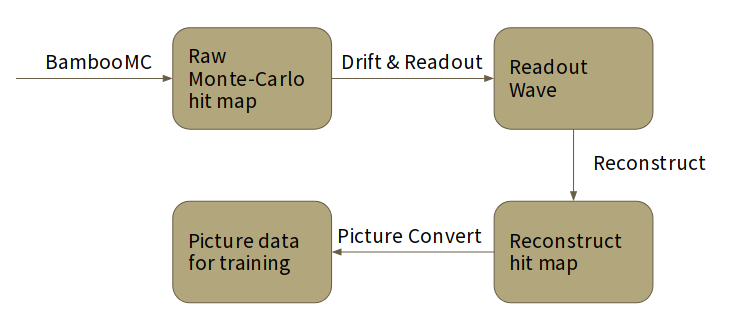
\includegraphics[width=0.6\columnwidth]{pic/process.png}
    \caption{模拟数据转换为CNN所需要的图片过程示意图。}
    \label{fig:process}
\end{figure}

\subsubsection{探测器响应}

    在 CNN 数据准备中对于探测器响应的处理和背景模拟中完全一致。

\subsubsection{读出结构}

    探测器两端各有一个读出平面,分别由 41 个 MM 读出板组件构成,如图\ref{fig:mms}所示。每个 MM 读出板的尺寸是 200$\times$200 mm$^2$,分别拥有 64 个 X 读出道 和 Y 读出道,总计探测器每端拥有 5248 个读出道。在处理过程中我们需要完整地构建读出平面结构以及 MM 读出板细节,从而能够精确得到读出平面(x,y)位置于所处通道的关联信息,并依次将漂移到读出平面上电离电子的位置时间信息(vector<x,y,t>)转换为波形信息(map<channel\_id, vector<count>>)。

    对于 MM 的处理中有一点需要注意,虽然 MM 的有效像素并没有完整的覆盖 $20\times20$cm$^3$ 的面积,但是因为电压是直接加在读出像素上的,那些位置不落在读出像素上的电子会在电场的作用下漂移到距离更近的像素。关于读出板的具体细节以及实现请参考 PandaXIII 中期报告\supercite{cdr}。

\subsubsection{电子学触发}

    这里使用了和前文背景模拟中一致的电子学参数: 采样率为 5MHz,采样点有 512 个,触发能量为 $Q_{\beta\beta}/2$。事实上电子学触发中关于触发能量的选择正是基于 NLDBD 事件的模拟数据,即我们希望通过选择最佳的触发能量使 NLDBD 事件的探测效率最高。图\ref{fig:trigger_select}中绘制了电子学触发能量对于 NLDBD 事件探测效率以及能量分辨率的影响,可以看出当触发能量位于 $Q_{\beta\beta}/2$ 附近时,通过触发的 NLDBD 事件效率最高。

    \begin{figure}
        \centering
        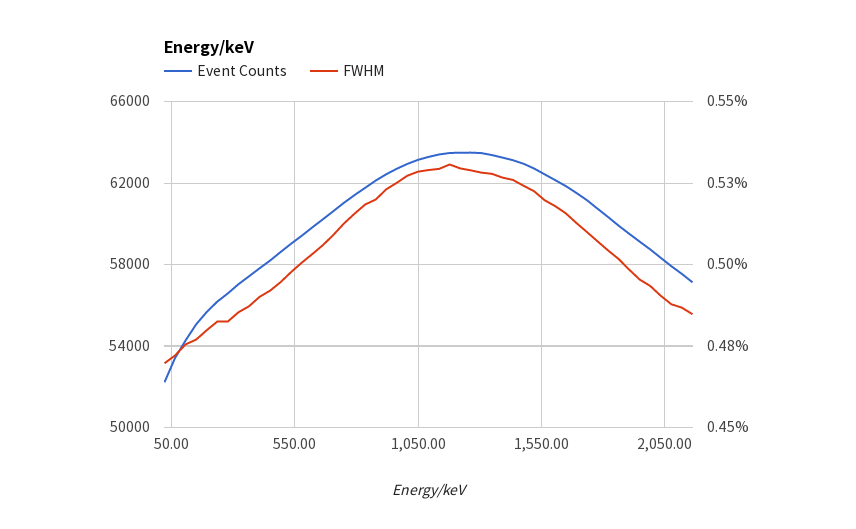
\includegraphics[width=0.8\columnwidth]{pic/trigger_select.png}
        \caption{电子学触发能量阈值对于 NLDBD 事件探测效率(蓝线,左轴)以及能量分辨率(红线,右轴)的影响。蓝线绘制了在 100000 个 NLDBD 事件中,达到触发的事件数目与触发能量阈值的关系,红线则是这些完成触发的 NLDBD 事件在 $Q_{\beta\beta}$ 处的能量分辨率。}
        \label{fig:trigger_select}
    \end{figure}

\subsubsection{重建}

    在考虑到探测器响应,读出结构以及电子学触发的相关影响后,原始模拟得到的 hit 信息已经被转换为了各个读出通道的波形信息,等价于真实探测器后采集到的数据格式。接下来便需要将波形信息重建回详细的事件径迹信息。

    对于一个事件中每个通道而言,X 或者 Y 坐标可以依据道数-位置关系得到 ,Z 坐标可以通过波形的时间信息和电子漂移速度计算得到,沉积能量可以通过对应时间点的强度信息(电子数目)和探测器$W$计算出。所以我们可以快速地将波形信息转换为两个二维直方图(Histogram),它在 Z 方向上有 512 个 bins ,间隔为 0.374mm,X 或者 Y 方向上最多有 448 个 bins ,间隔为 3mm,直方图的计数信息在代表着 bins 所对应的区域沉积能量的大小。

\subsubsection{图片转换}

    重建后得到的两个直方图即为事件在 X-Z-energy 和 Y-Z-energy 上的投影。我们分别计算出两个投影以能量为权重的位置重心,并以该位置为中心,按照 3mm 的尺寸重新划分(rebin)直方图,丢弃超过 $60\times60$ 范围外的数据信息。此时两个投影被转变为两个 $60\times60$ 尺寸的直方图,每个直方图又都可以映射为一张 $60\times60$ 像素的灰度图片,像素灰度的大小即代表着沉积能量的多少,其中能量最大的点所对应的灰度值为255。所以如同上文中所做的假设,在进行图片转换后事件总能量的信息以及 hit 的绝对位置信息都被抹去了。

    \begin{figure}
        \centering
        \begin{subfigure}[t]{0.22\textwidth}
          \centering
          \includegraphics[width=\textwidth]{pic/03_signal_3d_track.pdf}
          \caption{}
        \end{subfigure}
        \begin{subfigure}[t]{0.44\textwidth}
          \centering
          \includegraphics[width=\textwidth]{pic/03_signal_track.pdf}
          \caption{}
        \end{subfigure}
        \begin{subfigure}[t]{0.16\textwidth}
          \centering
          \setlength{\fboxsep}{0pt}
          \fbox{
\includegraphics[width=\textwidth]{pic/03_signal_final.png}}
          \caption{}
        \end{subfigure}
        
        \begin{subfigure}[t]{0.22\textwidth}
          \centering
          \includegraphics[width=\textwidth]{pic/03_background_3d_track.pdf}
          \caption{}
        \end{subfigure}
        \begin{subfigure}[t]{0.44\textwidth}
          \centering
          \includegraphics[width=\textwidth]{pic/03_background_track.pdf}
          \caption{}
        \end{subfigure}
        \begin{subfigure}[t]{0.16\textwidth}
          \centering
          \setlength{\fboxsep}{0pt}
          \fbox{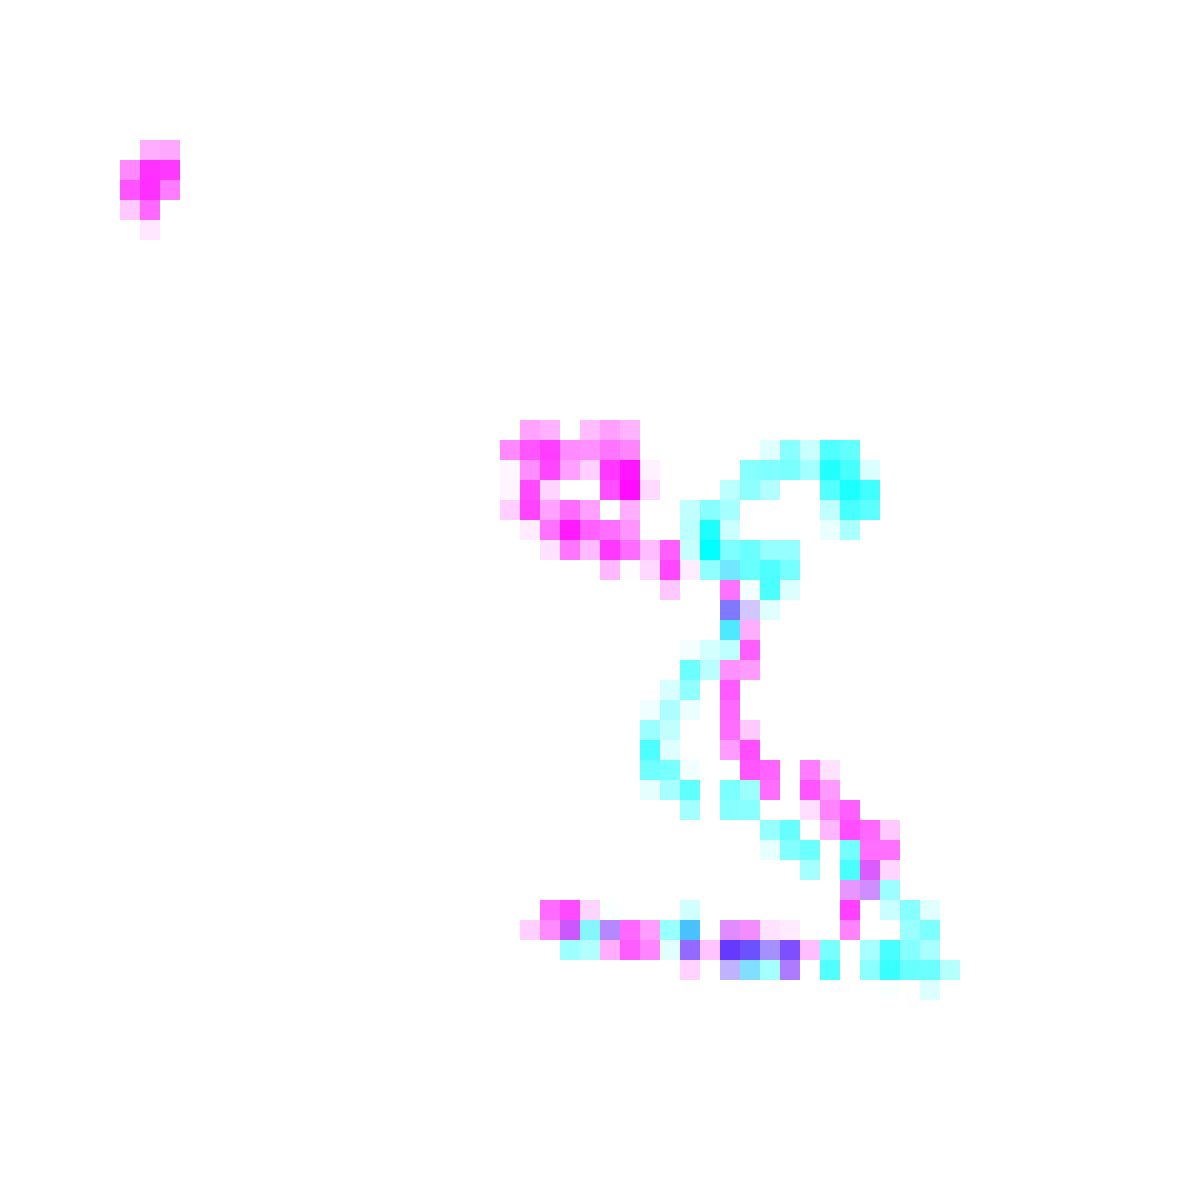
\includegraphics[width=\textwidth]{pic/03_background_final.png}}
          \caption{}
        \end{subfigure}
        
        \caption{NLDBD事件以及背景事件转换示意图。上部分:\xeots NLDBD 事件,下部分:2447keV $\gamma$ 本底事件。(a) 和 (d): BambooMC 模拟得到的原始 hit 信息。(b) 和 (e):重建后得到的 X-Z-energy 以及 Y-Z-energy 投影。(c) 和 (f):转换完成后的图片示意图,该图片并非 CNN 训练中所使用的图片,而是为了方便读者观看图片的颜色被后期处理过,其中青色代表着红色通道,粉红色代表着绿色通道。}
        \label{fig:image_mapping}
        \end{figure}

        
\subsubsection{数据转换总结}

图\ref{fig:image_mapping}举例示意了 NLDBD 事件及 $\gamma$ 本底事件的原始 hit 信息,重建后的投影信息和用于 CNN 训练的示意图片。我们一共模拟了1百万次 NLDBD 信号事件以及各 $2\times10^9$ 次
 2447keV 和 2614keV $\gamma$ 背景事件,经过上述各个转化过程后所生成的数据规模如表\ref{tab:convert}所示。

我们将使用CNN来进行二分类,所以信号和本底的数目应该保持对等,即各占 50\%。实验中背景是由两部分组成的,虽然根据之前的分析两种背景对于 CNN 而言应该是没有区别的,本文还是将它们混合共同作为 CNN 的背景样本,混杂的比例是 3.75:1,即无氧铜中 \utte 和 \thttt 放射性强度比。但需要注意的是,本文并没有研究该比例对实验结果的影响。我们一共准备了 $1.12\times10^6$ 组信号和背景数据图片,其中 80\% 被用于神经网络的训练过程中的训练部分(Training dataset),10\% 被用于训练过程中的验证部分(Validation dataset),最后的 10\% 用于后续的各种测试和检验(Check dataset)。
        
\renewcommand\arraystretch{1.4}
\begin{table*}
    \centering
    \begin{tabular*}{\textwidth}{@{\extracolsep{\fill}}ccccc}
        \hline
        \hline							
        	&	NLDBD	&	2447keV$\gamma$射线	&	2614keV$\gamma$射线	&	合计	\\
        \hline
        MC模拟事件数目	&	$1\times10^6$	&	$2\times10^9$	&	$2\times10^9$	&		\\
        总能量落入ROI事件数目	&	717163	&	3840611	&	1471989	&		\\
        漂移以及触发后事件数目	&	562959	&	1151395	&	485357	&		\\
        触发效率	&	78.50\%	&	30.00\%	&	33.00\%	&		\\
        总体探测效率	&	56.20\%	&	$5.76\times10^{-4}$	&	$2.43\times10^{-4}$	&		\\
        CNN图片数目	&	562959	&	444441	&	118517	&	1125917	\\
        \hline
        \hline
    \end{tabular*}
    \caption{NLDBD 信号样本以及 2447keV 和 2614keV 的 $\gamma$ 背景样本转换数据表。}
    \label{tab:convert}
  \end{table*}

\section{训练网络}
\label{section:train}

在完成数据准备后接下来的操作便是构建合适的 CNN 模型。可以说 CNN 模型的选择和调整是能否解决问题的关键,一个优秀的适合问题的模型可能可以带来极佳的分类效率和极小的分类误差。然而模型构建是一个非常困难的问题,在计算机学科中寻找到一个优秀的网络模型需要大量的计算,验证以及人工修正调整。因此在物理学中对 CNN 进行基本应用的过程中,优先使用现有模型并对其加以小的修正是一个较为经济和效率的事情。

我们在研究过程中测试并对比了多个神经网络模型,包括自己构建的简单的 3 层卷积神经网络模型,VGG16 模型\supercite{simonyan2014very}以及 Resnet50 模型\supercite{he2016deep}。我们使用了较小的数据集(约12.5\%的数据)对这三个模型进行了测试,最后选定 Resnet50 作为最终使用的模型。关于前两种模型的介绍以及三者的对比见附录\ref{section:resnet_compare}。

ResNet 被称作深度残差网络。在传统的卷积神经网络图像分类研究中,有一些相关的研究证明了越深的网络可能能够达到更佳的效果,但是单纯的叠加网络的层数会遇到梯度弥散的问题,即训练过程中样本对网络的回馈并不能有效的向上传递,导致部分网络层不能被有效地训练。ResNet 提出了如图\ref{fig:resnet}类似的结构,将输入 X 再次引入到输出,从而能够”跳过“部分层来降低训练造成的误差,这种连接方式被称作”快捷连接“(shortcut connection)。在本文中使用了有 50 个卷积层的 Resnet 网络作为主体结构,并对网络的输入层和输出部分做了简单的修改以满足我们的需求,网络的简单结构示意以及参数如表\ref{tab:resnet}所示。

\begin{figure}
    \centering
    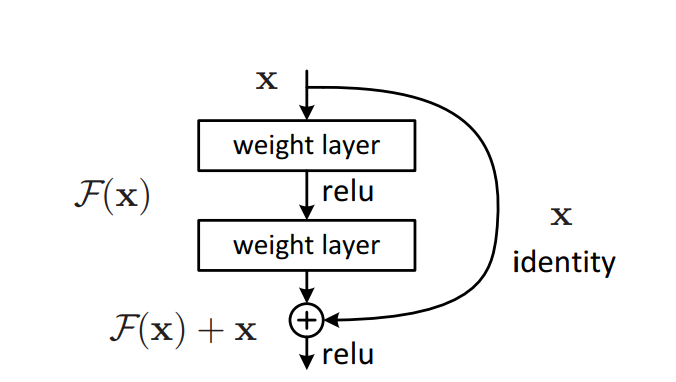
\includegraphics[width=0.6\columnwidth]{pic/resnet.png}
    \caption{Resnet 网络中快捷连接示意图,因为输入量 X 被直接引入到输出中,所以网络 $\mathcal{F}(X)$ 部分在训练过程中不会带来过多的误差。}
    \label{fig:resnet}
\end{figure}
\begin{table}
    \centering
    \begin{tabular}{ccccc}
      \\\hline \hline
  layer name & layer type &  output tensor  & layer attribute & repetition \\\hline \hline
  input\_1  & InputLayer & 240, 240, 3 &  & \\ \hline
  conv1 block & Convolution2D & 120, 120, 64 & 7$\times$7, 64 &  \\ \hline
  pooling & MaxPooling2D & 59, 59, 64 &  &  \\ \hline
  \multirow{3}{*}{conv2 block} & Convolution2D & 59, 59, 64 & 1$\times$1, 64 & \multirow{3}{*}3\\
   & Convolution2D & 59, 59, 64 & 3$\times$3, 64 & \\
   & Convolution2D & 59, 59, 256 & 1$\times$1, 256 & \\ \hline
  \multirow{3}{*}{conv3 block} & Convolution2D & 30, 30, 128 & 1$\times$1, 128 & \multirow{3}{*}{4} \\
   & Convolution2D & 30, 30, 128 & 3$\times$3, 128 & \\
   & Convolution2D & 30, 30, 512 & 1$\times$1, 512 & \\ \hline
  \multirow{3}{*}{conv4 block} & Convolution2D & 15, 15, 256 & 1$\times$1, 256 & \multirow{3}{*}{6} \\
   & Convolution2D & 15, 15, 256 & 3$\times$3, 256 & \\
   & Convolution2D & 15, 15, 1024 & 1$\times$1, 1024 & \\ \hline
  \multirow{3}{*}{conv5 block} &  Convolution2D & 8, 8, 512 & 1$\times$1, 512 & \multirow{3}{*}{3}\\
   & Convolution2D & 8, 8, 512 & 3$\times$3, 512 & \\
   & Convolution2D & 8, 8, 2048 & 1$\times$1, 2048 & \\ \hline
  pooling & AveragePooling2D & 1, 1, 2048 &  & \\ \hline
  flatten & Flatten & 2048 &  & \\ \hline
  dense & Dense & 256 & relu & \\  \hline
  dropout & Dropout & 256 &  & \\   \hline
  dense & Dense & 1 & sigmoid & \\ \hline \hline
    \end{tabular}
    \caption{修改后的 Resnet 网络结构示意表,表中“repetition”表示网络块重复堆叠的次数,默认是 1。网络中部分层以及快捷连接被省略,关于 Resnet50 核心部分的组成请参见论文\cite{he2016deep}。}
    \label{tab:resnet}
  \end{table}

我们使用 Keras\supercite{keras} 深度学习框架来构建和训练我们的 CNN 网络。Keras 使用 Python 作为框架的主要语言,并可以由 Google 公司推出的 Tensorflow\supercite{tensorflow} 张量计算框架做具体的张量计算。所以 Keras 可以应用由英伟达公司推出的 CUDA 显卡计算平台以及 cuDNN\supercite{cudnn} 库来加速训练的过程。我们在一台配置了 2 块 Nvidia Geforce 1080 显卡的工作站上进行了 30 轮(epochs\footnote{一轮是指所有的训练数据通过一次神经网络。})训练,每轮训练得到的权重信息都被保存了下来以供接下来的分析。在训练过程中为了降低过拟合,也对输入图片做了实时的数据提升,具体的训练细节见附录\ref{section:train_details}。训练总共耗时约5天。
  
\section{训练结果分析}
\label{section:cnn_result}

判断一个神经网络优劣的最为直观的指标之一便是准确度(accuracy),在分类模型中,它被定义为正确分类的样本数目与总样本数目的比值,用于标示该网络预测结果与真实结果的偏离程度。图\ref{fig:train_par}展示了在我们训练过程中,网络的准确度的变化趋势。可以看出随着训练的逐步进行,训练数据集的准确度不断增加。但在 20 轮后训练数据集的准确度明显超过了验证数据集,即发生了过拟合现象(overfit)。因此我们选择训练集和测试集准确度比较接近但又没有发生过拟合现象的几轮训练结果作为后续研究的对象,即第16轮到第20轮训练得到的网络权重。

\begin{figure}
    \centering
    \includegraphics[width=0.6\linewidth]{pic/04_resnet_tendency.pdf}
    \caption{训练过程中网络准确度随训练轮数变化的趋势。红色数据点表示训练数据集的准确度,蓝色数据点表示验证数据集的准确度。}
    \label{fig:train_par}
\end{figure}

在完成训练得到对应的网络权重后,便可以将权重加载到 CNN 网络模型中以预测未知的事件。通过上文的训练,我们得到了 5 组不同的网络权重,也就得到了 5 个 CNN 网络(后文称之为 Model-16 至 Model-20)。对于任一一个输入的事件图片,它们都可给出一个 0 到 1 之间的数 $\kappa$ ,表示该事件被 CNN 判断为更接近一个背景事件(0)或是一个信号事件(1)。图\ref{fig:cnn_dis}绘制了加载第 16 轮训练权重的网络(Model-16),预测测试数据集所得到的 $\kappa$ 分布。

\begin{figure}
    \centering
    \includegraphics[width=0.6\linewidth]{pic/05_resnet_distribution.pdf}
    \caption{Model-16 对于测试数据集的预测结果 $\kappa$ 分布图。当 $\kappa$ 接近 1 时背景事件的增多是因为的确有部分背景的径迹类似于 NLDBD 事件的径迹。}
    \label{fig:cnn_dis}
\end{figure}

单纯的使用准确度并不能较好的评价网络的效果,需要引入其他的评价方式来从上述 5 个网络中挑选出最好的一个。对于每个网络我们可以通过为 $\kappa$ 设置一个阈值 $\kappa_c$ 来区分背景和信号,这样就可以给出每个网络的信号以及背景效率曲线。图\ref{fig:cnn_eff}上半部分给出了 Model-16 的效率曲线。阈值的选择可以通过优化 FOM (figure of merit) 指标来完成,它一般被定义为最终探测到的信号的数目与背景数目开方的比值,即:
\begin{equation}
    FOM \propto \frac{s}{\sqrt{b}}=\frac{s_d}{\sqrt{b_d}}\cdot \frac{\epsilon_{s,cnn}}{\sqrt{\epsilon_{b,cnn}}}\propto \frac{\epsilon_{s,cnn}}{\sqrt{\epsilon_{b,cnn}}}
\end{equation}
其中 $\epsilon_{s,cnn}$ 和 $\epsilon_{b,cnn}$ 为在选定阈值 $\kappa_c$ 后网络的信号效率和背景效率,$s_d$ 和 $b_b$ 指在未经CNN网络处理前,探测器得到的信号数目以及背景数目。

\begin{figure}
    \centering
    \includegraphics[width=0.6\linewidth]{pic/06_efficiency.pdf}
    \caption{上半部分:Model-16 网络的信号效率(红线)以及背景拒绝效率(蓝线)随 $\kappa_c$ 变化图。下半部分:效率比 $\epsilon_{s,cnn}/\sqrt{\epsilon_{b,cnn}}$ 随 $\kappa_c$ 变化示意图。最优 $\kappa_c$ 位置由绿色虚线绘制出。}
    \label{fig:cnn_eff}
\end{figure}

PandaXIII 实验所能探测到的 NLDBD 事件半衰期与 FOM 成正比,所以可以通过最优化 $\epsilon_{s,cnn}/\sqrt{\epsilon_{b,cnn}}$ 来选择网络的 cut 位置 $\kappa_c$ 。图\ref{fig:cnn_eff}下半部分展示了 Model-16 中 $\epsilon_{s,cnn}/\sqrt{\epsilon_{b,cnn}}$ 随 $\kappa_c$ 的变化。当 $\kappa_c = 0.983$ 时,事件鉴别的 FOM 值最大。不同网络之间的优劣差别也可以通过对比最优 FOM 得到,表\ref{tab:efficiencies}描述了 Model-16 到 Model-20 5 种不同权重的网络 FOM 相关信息,从中可以看出 Model-16 能够达到最优的鉴别效果。此时信号效率为 47.5\%,背景拒绝率为 99.43\%,即压低本底约 175倍。

\begin{table}
    \centering
    \begin{tabular}{cccccc}
      \\\hline
      epoch & optimized $\kappa_c$ & $\epsilon_{s,cnn}$ & $ 1-\epsilon_{b,cnn}$ &$\epsilon_{s,cnn}/\sqrt{\epsilon_{b,cnn}}$ & final BI\\\hline
      16 & 0.983 & 0.475 & 0.9943 & 6.264 & $1.775\times10^{-5}$ \\
      17 & 0.976 & 0.569 & 0.9916 & 6.196 & $2.605\times10^{-5}$ \\
      18 & 0.981 & 0.487 & 0.9936 & 6.098 & $1.968\times10^{-5}$ \\
      19 & 0.966 & 0.540 & 0.9923 & 6.165 & $2.369\times10^{-5}$ \\
      20 & 0.976 & 0.520 & 0.9928 & 6.145 & $2.215\times10^{-5}$ \\\hline
      average &  &  &  & $6.174\pm0.055$ \\\hline
  %    std. err. &  & &  & 0.055 \\\hline
    \end{tabular}
    \caption{不同权重网络的最优 $\kappa_c$ 以及对应的信号效率 $\epsilon_{s,cnn}$,背景拒绝率 $1-\epsilon_{b,cnn}$,$\epsilon_{s,cnn}/\sqrt{\epsilon_{b,cnn}}$ 和最终的本底水平(BI,单位:count$\cdot$kg$^{-1}\cdot$keV$^{-1}\cdot$year$^{-1}$)。BI 计算过程中使用了 $3.088\times10^{-3}$ count$\cdot$kg$^{-1}\cdot$keV$^{-1}\cdot$year$^{-1}$ 作为未经 CNN 网络鉴别时的本底水平。}
    \label{tab:efficiencies}
  \end{table}
  
从表中数据来看虽然各个模型中选取最优阈值时信号效率以及背景拒绝率率相差较大,但是其比值 $\epsilon_{s,cnn}/\sqrt{\epsilon_{b,cnn}}$ 十分的稳定,误差只有约 0.1\%。这说明使用 CNN 来进行事件鉴别还是相对稳定的,其达到的最终效果与模型的结构关系较大,而与训练的次数关系较小。在这些网络中,我们最终选定了效果最好的 Model-16 权重网络作为 PandaXIII 事件鉴别中所用的网络。图\ref{fig:cnn_roc}绘制了该网络的 ROC 曲线。图\ref{fig:cnn_specturm}绘制了经过 Model-16 分类前后,测试数据集的能谱对比图,该能谱对比图也验证了之前 CNN 并不使用总能量来判断事件的猜想。对于前文中另外的一个假设,我们使用了 Model-16 测试了部分产生自螺钉的背景信号,得到了一致的鉴别效率,即认为本底的生成位置对我们的研究没有影响。

\begin{figure}
    \centering
    \includegraphics[width=0.6\linewidth]{pic/06b_roc.pdf}
    \caption{Model-16 背景拒绝率与信号效率关系图(ROC曲线)}
    \label{fig:cnn_roc}
\end{figure}

\begin{figure}
    \centering
    \includegraphics[width=0.8\linewidth]{pic/08_energy_spectrum.pdf}
    \caption{经过 CNN 鉴别前后,信号以及背景的能谱对比示意图。左图:NLDBD 信号事件。右图:2447keV $\gamma$ 背景事件。}
    \label{fig:cnn_specturm}
\end{figure}

正如图\ref{fig:cnn_dis}分布中所绘制的,虽然 CNN 的分类效果十分优异,但是仍然有一部分的误判存在。图\ref{fig:wrong_judge}给出了两个被错误分类事件的投影图。但是在这两个误判事例中 NLDBD 事件的径迹看上去的确只有一个布拉格峰,而背景事件也确实发生了连续的两次康普顿散射过程从而使得径迹拥有两个明确的布拉格峰。因此我们认为的确有一部分背景事件的物理特征就如同NLDBD事件一样,从而使得 CNN 做出了错误判断。这也解释了图\ref{fig:cnn_dis}中背景事例 $\kappa$ 的分布为什么不是单调递减,而是在靠近 1 时由一个较小的上升。

\begin{figure}
    \centering
    \includegraphics[width=0.8\linewidth]{pic/07_sab_track.pdf}
    \includegraphics[width=0.8\linewidth]{pic/07_bas_track.pdf}
    \caption{使用 Model-16 错误分类的一些事件投影图。上图:一个被认为成背景的 NLDBD 信号事件,下图:一个被认为成信号的背景事件。}
    \label{fig:wrong_judge}
\end{figure}

\section{小结}

本章研究了使用 CNN 深度卷积神经网络鉴别蒙特卡洛产生的 NLDBD 事件和背景事件。通过使用 Resnet50 网络模型我们能够在压低背景信号 175 倍的同时达到 47.5\% 的信号效率。PandaXIII 中期报告中给出 NLDBD 事件半衰期检测线满足公式\ref{eq:half}\supercite{cdr}
\begin{equation}
    T_{1/2}^{0\nu}\propto\eta\cdot\epsilon\sqrt{\frac{M\cdot T}{r\cdot\delta E}}
    \label{eq:half}
\end{equation}
其中 $\eta$ 为探测器效率,r 为本底水平 BI,即正比与上文中提到的FOM 。相较于设计报告中对于事件鉴别的预期(压低本底 30-35 倍时达到 35\% 的探测效率)CNN 完满的完成了目标,并能够额外带来 64.2\% 的提升,如表\ref{tab:comparison}所示。按照中期报告中对于检测线的估算并考虑到 CNN 对其带来的提高,在使用 1 吨量级探测采样 3 年后,PandaXIII 实验 \xeots NLDBD 的半衰期检测线可以达到约 $1.6\times10^{27}$ 年。

\begin{table}[hbt]
    \centering
    \begin{tabular}{ccccc}
      \\\hline
      & PandaX-III 基准 & CNN (model-16) & CNN (model-18) & CNN (average) \\\hline
      $\epsilon_{s}$ & 0.645 & 0.475  & 0.487 & \\
      $ 1-\epsilon_{b}$ & 0.9714 & 0.9943  & 0.9936 &\\
      $\epsilon_{s}/\sqrt{\epsilon_{b}}$ & 3.816 & 6.264 & 6.098 & 6.174 \\\hline
      改进 & - & $64.2\%$ & $59.8\%$ & $61.8\%$\\\hline
    \end{tabular}
    \caption{使用CNN鉴别事件与PandaXIII中期报告中基准设计对比表。}
    \label{tab:comparison}
  \end{table}
  

% vim:ts=4:sw=4
